\documentclass[11pt]{article}
\usepackage[margin=1in]{geometry}
\usepackage{booktabs}
\usepackage{pgfplots}
\pgfplotsset{compat=1.18}
\begin{document}
\section*{DOOM Quality Modernization: Before vs. After}

This report uses an additive policy. The general host/native profile is not
replaced by the guest-C profile, and future \texttt{malbolge-*} checks will add
to the result rather than erase existing diagnostics.

The generated corpus is clean for the current guest-C bootstrap and for all
390 strict compiler checks. It is not clean under the repository's complete
general profile: 36,686 unique findings remain. Those findings are retained
and classified below instead of being relabeled as zero.

Before corpus: \texttt{doom}.\\
After corpus:
\texttt{algorithms/doom/quality/out/doom\_fixed}.\\
Pinned validator toolchain: LLVM/Clang 22.1.8.

\subsection*{Corpus metrics}
\begin{tabular}{lrr}
\toprule
Metric & Before & After \\
\midrule
C translation units & 72 & 65 \\
Headers & 74 & 84 \\
All files & 166 & 151 \\
Physical source lines & 59110 & 78605 \\
Nonblank source lines & 48963 & 70182 \\
Source bytes & 1333724 & 2474438 \\
WAD files & 1 & 1 \\
WAD bytes & 28795076 & 28795076 \\
\bottomrule
\end{tabular}

WAD files are test data and are excluded from source line and byte metrics.

\subsection*{Additive validation verdict}
\begin{tabular}{lrrl}
\toprule
Gate & Checks or units & Findings & Status \\
\midrule
Guest-C bootstrap & 65 units & 0 & clean \\
Strict compiler matrix & 390 checks & 0 & clean \\
General host/native profile & 65 units & 36686 & not clean \\
Combined current policy & --- & 36686 & not clean \\
\bottomrule
\end{tabular}

The guest bootstrap currently uses stock Clang checks. The project-owned
\texttt{malbolge-*} plugin is not implemented yet. When available, its findings
will be added to the general count.

\subsection*{General-profile outcome}
\begin{tabular}{lrrr}
\toprule
Metric & Before & After & Reduction (\%) \\
\midrule
Unique findings & 143662 & 36686 & 74.46 \\
Raw reports & 201160 & 96861 & 51.85 \\
Findings / KLOC & 2430.42 & 466.71 & 80.80 \\
\bottomrule
\end{tabular}

\subsection*{Findings by general gate}
\begin{tabular}{lrr}
\toprule
Gate & Before & After \\
\midrule
clang-format & 75797 & 697 \\
clang-linux-arm64 & 3 & 0 \\
clang-linux-x86\_64 & 2497 & 0 \\
clang-tidy & 43619 & 35616 \\
editorconfig & 21720 & 370 \\
interop heuristic & 26 & 3 \\
\bottomrule
\end{tabular}

\subsection*{Why 36,686 findings remain}
\begin{tabular}{lrl}
\toprule
Class & Count & Interpretation \\
\midrule
Literal and table constants & 22304 & strict policy debt \\
Historical naming and length & 3313 & source/linkage migration \\
Braces, includes, format, text & 4746 & mechanical debt \\
Signed bitwise operations & 1461 & priority portability review \\
Initialization and globals & 2700 & architectural debt \\
Remaining rules & 2162 & mixed review debt \\
\bottomrule
\end{tabular}

The 22,304 magic-number reports are dominated by renderer tables, fixed-point
constants, protocol values, and historical game data. They are real violations
of the configured rule, but they are not 22,304 independent runtime defects.
A compliant repair needs named domain constants or generated data tables.

Naming and identifier-length findings cover historical APIs and pervasive
short mathematical names. Bulk renaming would be a large source and linkage
migration, not a compatibility fix.

Braces, direct includes, formatting, and text layout are actionable mechanical
debt. They remain counted because no blanket suppression is accepted.

Signed bitwise findings deserve the highest correctness priority. Many sites
are deliberate fixed-point or bit-level operations, but each still needs an
unsigned-domain proof or rewrite. Analyzer and bugprone findings in the
remaining class likewise require individual review.

Initialization, mutable-global, complexity, and function-size rules challenge
the original DOOM architecture. Satisfying them requires structural
modernization beyond the completed source-bound compatibility transform.

The three interoperability heuristic findings are not equivalent to missing
host support. Two expect platform-specific Windows/macOS source inside the
guest tree, while the accepted design exposes one host-neutral capability ABI.
The third is a stale \texttt{sndserver} comment. They remain visible until the
heuristic or source text is corrected.

\subsection*{Visual comparison}
\begin{center}
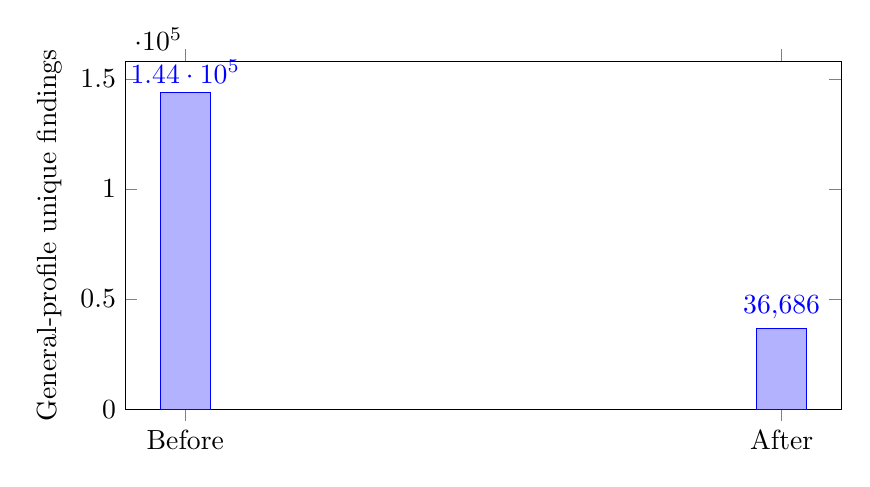
\begin{tikzpicture}
\begin{axis}[
ybar,
bar width=18pt,
width=0.88\linewidth,
height=6cm,
ylabel={General-profile unique findings},
symbolic x coords={Before,After},
xtick=data,
nodes near coords,
ymin=0,
]
\addplot coordinates {(Before,143662) (After,36686)};
\end{axis}
\end{tikzpicture}
\end{center}

\subsection*{Reproducibility}
Before source SHA-256:
\texttt{a7c20cd5bcdad32c87a85d855b2a77c63be5591ebf8186550436e75587d72ec7}.\\
After source SHA-256:
\texttt{b05238614b21080b55a4e0e113a1369a69548217bded480dcdacdae5af3f1d70}.\\
Before asset SHA-256:
\texttt{23dbc435d8be77ce4db134954581a293309c275c39f95f38cc8cf0df084044fa}.\\
After asset SHA-256:
\texttt{23dbc435d8be77ce4db134954581a293309c275c39f95f38cc8cf0df084044fa}.\\
Machine-readable metrics:
\texttt{algorithms/doom/quality/comparison/metrics.json}.

The report stores aggregate evidence only and intentionally omits a
per-finding ledger.
\end{document}
